\section{Jordfugt Design} \label{sec:Jordfugt_Design}

Dette afsnit omhandler design af blokken Jordfugt, der består af et PSoC4 Pioneer kit og 0-6 jordfugtsensorer. 

\begin{figure}[h]
\centering 
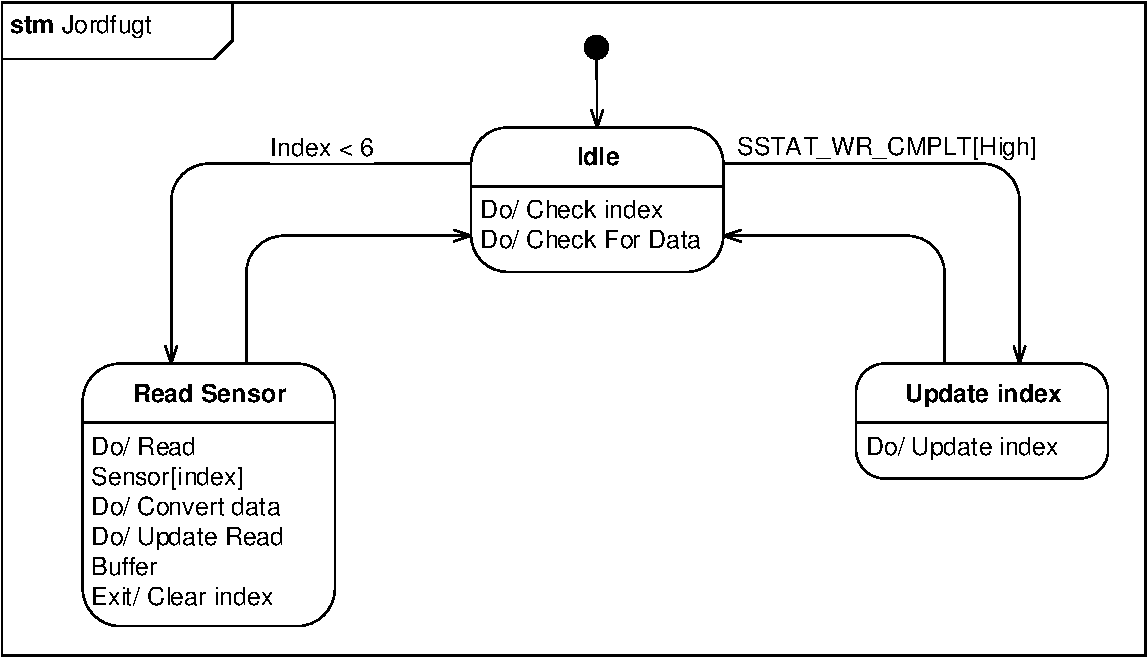
\includegraphics[width={\textwidth}, trim=0 0 0 0, clip=true] {../fig/stm_jordfugt.pdf}
\caption{State Machine for SW på PSoC4 i blokken Jordfugt}
\label{fig:stm_jordfugt}
\end{figure}

Ovenstående figur (Figur \ref{fig:stm_jordfugt}) viser en state machine for SW i PSoC4 i blokken Jordfugt.
 
PSoC'en står hele tiden og poller på om der er modtaget data, og om en indexvariabel er mindre end 6, som er det maximale antal jordfugtsensorer, der kan tilkobles.

Såfremt der er modtaget data via \IIC komminukationen, opdateres index variablen til det sensornummer, der er modtaget. 

Såfremt index variablem er mindre end 6, læses der på den tilhørende sensor, data konverteres til et tal mellem 1 - 100, og read bufferen opdateres med den læste værdi. 

\mbox{}

Der er i forbindelse med brugen af sensoren lavet en støjundersøgelse i faget Mixed Signal Elektronik. 
Se journalen \cite{lib:MSE_06} for nærmere info. 
I AutoGreen anvendes jordfugtsensoren på en noget simplere måde end i øvelsen, se afsnittet om implementering af blokken Jordfugt for nærmere info.

\clearpage